\documentclass{article}
\usepackage[utf8]{inputenc} % UTF-8
\usepackage{amsmath}
\usepackage{amssymb}
\usepackage{algpseudocode} % Algoritmos
\usepackage[a4paper, total={6in, 8in}]{geometry}
\usepackage{graphicx} % Figuras e imagenes
\usepackage{multirow} % Combinacion de celdas en tablas
\usepackage{algorithmicx}
\usepackage{fancyhdr} % Cabeceras y pies de pagina
\graphicspath{ {images/} } % Ruta a las imagenes

\title{Práctica 2 - Complejidad de $\mathcal{H}$ y modelos lineales}
\author{Luis Miguel Guirado Bautista - Universidad de Granada}
\date{1 de Mayo de 2022}

\pagestyle{fancy}
\fancyhf{}

% do-while en algoritmos
\algdef{SE}[DOWHILE]{Do}{doWhile}{\algorithmicdo}[1]{\algorithmicwhile\ #1}%

\renewcommand*\contentsname{Índice} % Nombre del indice
\renewcommand{\figurename}{Figura} % Nombre de una figura
\renewcommand{\partname}{Ejercicio} % Nombre de \part
\renewcommand{\familydefault}{\sfdefault}

\begin{document}

    \begin{titlepage}
        \maketitle
        \thispagestyle{empty}
    \end{titlepage}

    \pagebreak

    \lhead{Práctica 2 - Complejidad de $\mathcal{H}$ y modelos lineales}
    \rhead{Luis Miguel Guirado Bautista}
    \tableofcontents

    \pagebreak
    \rfoot{\thepage}
    \section{Complejidad de $\mathcal{H}$ y el ruido}

    \subsection*{Funciones usadas}

    \begin{enumerate}
        \item[-]\texttt{simula\_unif(N, dim, rango)} \par 
        Genera \texttt{N} vectores aleatorios uniformes de dimensión \texttt{dim}.
        dentro del \texttt{rango}

        \begin{figure}[h]
            \centering
            \caption{Datos generados por \texttt{simula\_unif(N=50, dim=2, rango=[-50,50])}}
            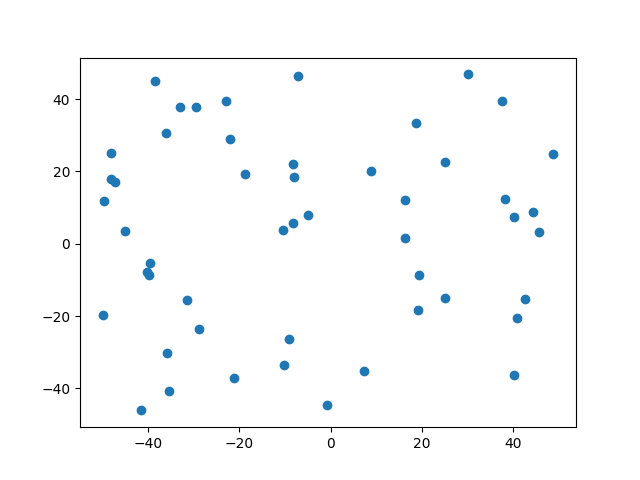
\includegraphics[width=\textwidth]{uniform.png}
        \end{figure}
        \pagebreak
        \item[-]\texttt{simula\_gauss(N, dim, sigma)} \par
        Genera \texttt{N} vectores aleatorios  de dimensión \texttt{dim} dentro de una distribución Gaussiana.

        \texttt{sigma} es un vector de dimensión \texttt{dim} que posee el valor de la varianza en la
        distribución Gaussiana para cada una de las dimensiones.
        \begin{figure}[h]
            \centering
            \caption{Datos generados por \texttt{simula\_gauss(N=50, dim=2, sigma=[5,7])}}
            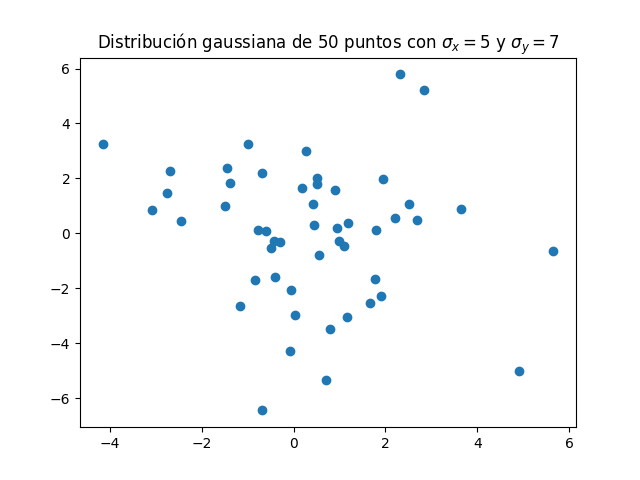
\includegraphics[width=\textwidth]{gauss.png}
        \end{figure}
        \pagebreak
        \item[-]\texttt{simula\_recta(intervalo)} \par
        Simula una recta del tipo $y = ax + b$ aleatoria con valores dentro de \texttt{intervalo}.

        Devuelve los coeficientes $a$ y $b$.
        \begin{figure}[h]
            \centering
            \caption{Datos generados por \texttt{simula\_recta(intervalo=[-50,50])}}
            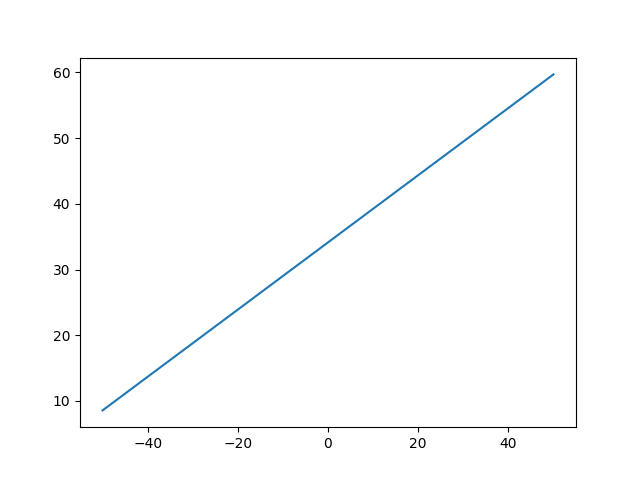
\includegraphics[width=\textwidth]{recta.png}
        \end{figure}
    \end{enumerate}
    \pagebreak

    \subsection{Influencia del ruido en la selección de la complejidad de $\mathcal{H}$}

    Vamos a generar una muestra aleatoria uniforme con \texttt{simula\_unif(100, 2, [-50,50])}, y vamos a
    clasificar los puntos según la siguiente función:

    \begin{equation*}
        f(x, y) = sign(y - ax - b)
    \end{equation*}

    Donde la tupla $(x,y)$ representa las coordenadas del punto de la función y la tupla $(a,b)$
    representa los coeficientes de la recta $ax + b$, generados por la función \texttt{simula\_recta}.

    \pagebreak

    \section{Modelos lineales}

    \subsection{Algoritmo Perceptrón (PLA)}

    \pagebreak

    \subsection{Regresión Logística (RL)}

    \pagebreak

    \section{Bonus. Clasificación de dígitos.}

\end{document}